\section{函数的概念}

关于函数的概念,在中学数学中我们已经有了初步的了解,本节将对此作进一步的讨论.

\subsection{函数的定义}

\begin{definition}[函数]\label{def:fx}
    给定两个实数集 $D$ 和 $M$, 若有对应法则 $f$, 使得对于每一个 $x\in D$,都有唯一的 $y\in M$与它相对应,则称 $f$ 是定义在数集 $D$ 上的\textbf{函数} ,记作    
    \begin{align} \label{eq:fx}
        f  :&D \to M\notag \\ 
        &x  \longmapsto y
    \end{align}
    数集 $D$ 称为函数 $f$ 的\textbf{定义域},$x$ 所对应的 $y$ 称为 $f$ 在点 $x$ 处的\textbf{函数值},常记为 $f(x)$. 全体函数值的集合 $f(D)=\{ y \mid y=f(x),x \in D\}\subset M$ 称为函数 $f$ 的\textbf{值域}.
\end{definition}

\eqtref{eq:fx} 中的第一式 “$f:D\to M$”表示按照法则 $f$ 建立数集 $D$ 到 $M$ 的函数关系;第二式“$x\longmapsto y$ 表示这两个数集中元素之间的对应关系,也可以记作 “$x\longmapsto f(x)$”.习惯上,我们称此函数关系中的 $x$ 为\textbf{自变量},$y$ 为\textbf{因变量}.

关于函数的定义,我们作如下几点说明:

\begin{enumerate}
    \item \defref{def:fx}中的实数集 $M$ 常用 $\R$ 来代替,于是定义域 $D$ 和对应法则 $f$ 就成为确定函数的两个主要因素.所以,我们也常用 $y=f(x),x\in D$ 来表示一个函数.由此,我们说某两个函数相同,是指它们有相同的定义域和对应法则.如果两个函数对应法则相同而定义域不同,那么这两个函数仍然是不相同的.例如 $f(x)=1,x\in \R$ 和 $g(x)=1,x\in \R\backslash\{0\}$ 是不相同的两个函数.另一方面,两个相同的函数,其对应法则的表达形式可能有所不同.例如 $\varphi(x)=\abs{x},x\in R$ 和 $\psi (x)=\sqrt{x^2},x\in \R$.
    \item 我们在中学数学中已经知道,表示函数的主要方法是解析法(公式法),即用数学运算式子来表示函数.这时,函数的定义域常取使得该运算式子有意义的自变量的全体,通常称为\textbf{存在域}.在这种情况下,函数的定义域(即存在域)$D$ 可以省略不写,而只用对应法则 $f$ 来表示一个函数,此时可以简单地说“函数 $y=f(x)$” 或“函数$f$”.
    \item 函数 $f$ 给出了 $x$ 轴上的点集 $D$ 到 $y$ 轴上的点集 $M$ 之间的\textbf{单值对应},也称为\textbf{映射}.对于 $a\in D$,$f(a)$ 称为映射 $f$ 下 $a$ 的\textbf{象},$a$ 则称为 $f(a)$ 的\textbf{原象}.
    \item 在函数定义中,对每一个 $x\in D$ ,只能有唯一的一个 $y$ 值与之对应,这样定义的函数称为 \textbf{单值函数}.若同一个 $x$ 值可以对应多于一个的 $y$值,则称这种函数为 \textbf{多值函数}.在本书范围内,我们只讨论单值函数.
\end{enumerate}

\subsection{函数的表示法}

在中学课程里,我们已经知道函数的表示法主要有三种,即解析法、列表法和图像法.

有些函数在其定义域的不同部分用不同的公式表达,这类函数通常称为\textbf{分段函数}.例如,函数
\[
\sgn x=\begin{cases}
    1,& x>0 \\
    0,&x=0 \\
    -1,&x<0 \\
\end{cases}
\]是分段函数,称为\textbf{符号函数},其图像如\figref{fig:sign}所示.又如函数 $f(x)=\abs{x}$ 也可以用如下的分段函数表示:
\[
f(x)=\begin{cases}
    x, & x\ge 0 \\ 
    -x,& x<0
\end{cases}
\]
它还可以表示为 $f(x)=x\sgn x$.

\begin{figure}[htbp]
\centering
\begin{tikzpicture}
 \draw[->] (-2.5,0)--(2.5,0) node[below] {$x$};
 \draw[->] (0,-2)--(0,2) node[above] {$y$};
 \draw[red,smooth,thick,samples=50,domain=-2:0] plot(\x,-1);
 \draw[green,smooth,thick,samples=50,domain=0:2] plot(\x,1);
 \filldraw[blue] (0,0) circle(2pt);
 \draw[green] (0,1) circle(2pt);
 \draw[red] (0,-1) circle(2pt);
 \node[anchor=north west] at (0,0){$O$};
 \node[anchor=east] at (0,1) {$1$};
 \node[anchor=west] at (0,-1) {$-1$};
\end{tikzpicture}
\caption{$\sgn x$ 的图像}
\label{fig:sign}
\end{figure}

函数 $y=f(x),x\in D$ 又可以用有序数对的集合 $G=\{(x,y)\mid y=f(x),x\in D\}$ 来表示.在坐标平面上,集合 $G$ 的每一个元素 $(x,y)$ 对应平面上的一个点,因而集合 $G$ 在坐标平面上描绘出这个函数的图像.这就是用图像法表示函数的依据.

有些函数只能用语言来描述.比如,定义在 $\R$ 上的狄利克雷( Dirichlet) 函数
\[
D(x) = \begin{cases}
    1,& \mbox{当} x \mbox{为有理数} \\ 
    0,& \mbox{当} x \mbox{为无理数}
\end{cases}
\]
和定义在 $[0,1]$ 上的黎曼(Riemann)函数
\[
R(x)=\begin{cases}
    \frac{1}{q},& \mbox{当}  x =\frac{q}{p}(p,q\in \N_+,\frac{q}{p} \mbox{为既约真分数} )\\
    0,& \mbox{当}x=0,1\mbox{和}(0,1)\mbox{内的无理数}.
\end{cases}
\]
\figref{fig:liman}是这两个函数的示意图.

\begin{figure}
    \begin{minipage}{0.46\textwidth}
        \begin{tikzpicture}
            \draw[->] (-3,0)--(3,0) node[below] {$x$};
            \draw[->] (0,-2)--(0,2) node[left] {$y$};
            \draw[dotted,thick,red] (-2.9,0)--(2.9,0);
            \draw[dotted,thick,green] (-2.9,1)--(2.9,1);
            \node[anchor=north west] at (0,0){$O$};
            \node[anchor=south east] at (0,1) {$1$};
        \end{tikzpicture}
    \end{minipage}
    \hfill
    \begin{minipage}{0.46\textwidth}
        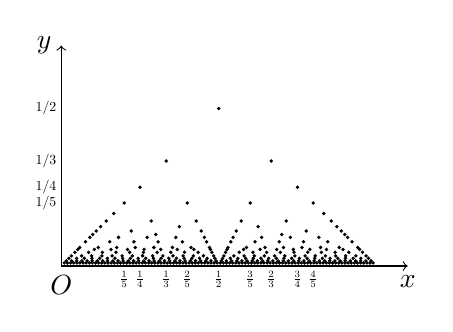
\begin{tikzpicture}[scale=4]
            \draw[->] (0,0)--(1.1,0) node[below] {$x$};
            \draw[->] (0,0)--(0,0.7) node[left] {$y$};
            \node[anchor=north] at (0,0){$O$};
            \foreach \q in {1,2,3,...,100} \draw (\q/101,1/101) circle(0.1pt);
            \foreach \q in {1,2,3,...,60} \draw (\q/61,1/61) circle(0.1pt);
            \foreach \q in {1,2,3,...,40} \draw (\q/41,1/41) circle(0.1pt);
            \foreach \q in {1,2,3,...,30} \draw (\q/31,1/31) circle(0.1pt);
            \foreach \q in {1,2,3,...,22} \draw (\q/23,1/23) circle(0.1pt);
            \foreach \q in {1,2,3,...,18} \draw (\q/19,1/19) circle(0.1pt);
            \foreach \q in {1,2,3,...,16} \draw (\q/17,1/17) circle(0.1pt);
            \foreach \q in {1,2,3,...,12} \draw (\q/13,1/13) circle(0.1pt);
            \foreach \q in {1,2,3,4,5,6,7,8,9,10} \draw (\q/11,1/11) circle(0.1pt);
            \foreach \q in {1,3,7,9} \draw (\q/10,1/10) circle(0.1pt);
            \foreach \q in {1,2,4,5,7,8} \draw (\q/9,1/9) circle(0.1pt);
            \foreach \q in {1,3,5,7} \draw (\q/8,1/8) circle(0.1pt);
            \foreach \q in {1,2,3,4,5,6} \draw (\q/7,1/7) circle(0.1pt);
            \foreach \q in {1,5} \draw (\q/6,1/6) circle(0.1pt);
            \foreach \q in {1,2,3,4} \draw (\q/5,1/5) circle(0.1pt);
            \foreach \q in {1,3} \draw (\q/4,1/4) circle(0.1pt);
            \foreach \q in {1,2} \draw (\q/3,1/3) circle(0.1pt);
            \foreach \q in {1} \draw (\q/2,1/2) circle(0.1pt);
            \foreach \q in {1,2,3,4} \draw node[scale=0.5,below] at (\q/5,0) {$\frac{\q}{5}$};
            \foreach \q in {1,3} \draw node[scale=0.5,below] at (\q/4,0) {$\frac{\q}{4}$};
            \foreach \q in {1,2} \draw node[scale=0.5,below] at (\q/3,0) {$\frac{\q}{3}$};
            \foreach \q in {1} \draw node[scale=0.5,below] at (\q/2,0) {$\frac{\q}{2}$};
            \foreach \p in {2,3,4,5} \draw node[scale=0.5,left] at (0,1/\p) {1/\p};
        \end{tikzpicture}
    \end{minipage}
    \caption{狄利克雷函数和黎曼函数的示意图}
    \label{fig:liman}
\end{figure}

\subsection{函数的四则运算}

\begin{definition}[函数的四则运算]
    给定两个函数 $f,x\in D_1$ 和 $g,x\in D_2$. 记 $D=D_1 \cap D_2$,并设 $D\ne \varnothing$.我们定义 $f$ 与 $g$ 在 $D$ 上的和、差、积运算如下:
    \begin{align*}
        F(x)&=f(x) + g(x),x\in D \\
        G(x)&=f(x) - g(x),x\in D \\
        H(x)&=f(x)g(x),x\in D 
    \end{align*}
    若在 $D$ 中剔除使$g(x)=0$的$x$值,即令$D^*=D_1\cap \{x\mid g(x)\ne 0,x\in D_2\}\ne \varnothing$,可在 $D^*$ 上可以定义 $f$ 与 $g$ 的商的运算如下:
    \[
    L(x)=\frac{f(x)}{g(x)},x\in D^*
    \]
\end{definition}

\begin{annotation}
    若 $D=D_1 \cap D_2=\varnothing$,则$f$ 与 $g$ 不能进行四则运算.例如,设
    \begin{align*}
        f(x)&=\sqrt{1-x^2},x\in D_1 = \setset{x}{\abs{x}\le 1} \\
        g(x)&=\sqrt{x^2-4},x\in D_2 = \setset{x}{\abs{x}\ge 2} 
    \end{align*}
    由于 $D=D_1 \cap D_2=\varnothing$,所以表达式 $f(x) + g(x)=\sqrt{1-x^2}+\sqrt{x^2-4}$是没有意义的.
\end{annotation}

以后为了叙述方便,函数 $f$ 与 $g$ 的和、差、积、商分别写作 $f+g,f-g,fg,\frac{f}{g}$.

\subsection{复合函数}
\begin{definition}[函数的复合]
    设有两个函数 $y=f(u),u\in D$ 和 $u=g(x),x\in E$. 记 $E^*=\setset{x}{g(x)\in D} \cap E$.若 $E^*\ne \varnothing
$,则对每一个 $x\in E^*$,都可以通过函数 $g$ 对应 $D$ 上唯一的一个值 $u$ ,而 $u$ 又可以通过函数 $f$ 对应唯一的一个值 $y$.这就确定了一个定义在$E^*$ 上的函数,它以$x$为自变量,$y$为因变量,记作 
    \begin{center}
        $y=f(g(x)),x\in E^*$ 或 $(f\circ g)(x),x\in E^*$ 
    \end{center}称为函数 $f$ 与 $g$ 的\textbf{复合函数},并称 $f$ 为\textbf{外函数},$g$ 为\textbf{复合函数},$u$ 为\textbf{中间变量}.
\end{definition}

函数 $f$ 与 $g$ 的复合运算也可以简单地写作$f\circ g$.

\begin{example}
    求函数 $y=f(u)=\sqrt{u},u\in D=[0,+\infty)$ 与函数 $u=g(x)=1-x^2,x\in E=\R$ 的复合函数.
\end{example}

\begin{solve}
    定义域 $E^*=\setset{x}{1-x^2\ge 0} \cap \R=[-1,1]$.

    复合函数为$y=f(g(x))=\sqrt{1-x^2},x\in E^*$ 或 $(f\circ g)(x)=\sqrt{1-x^2},x\in E^*$ 
\end{solve}

复合函数也可以由多个函数相继复合而成.例如,由三个函数 $y=\sin u,u=\sqrt{v},v=1-x^2$ (它们的定义域取为各自的存在域)相继复合而得的复合函数为 $y=\sin \sqrt{1-x^2},x\in [-1,1]$.

\begin{annotation}
    当且仅当 $E^*\ne \varnothing$ 时, 函数 $f$ 与 $g$ 才能进行复合.例如,以 $y=f(u)=\arcsin u,u\in D=[-1,1]$ 为外函数, $u=g(x)=2+x^2,x\in E=\R$ 为内函数,就不能进行复合.这是因为外函数的定义域 $D=[-1,1]$ 与内函数的值域 $g(E)=[2,+\infty)$不相交.
\end{annotation}

\subsection{反函数}

函数 $y=f(x)$ 的自变量 $x$ 与因变量 $y$ 的关系往往是相对的.有时我们不仅要研究 $y$ 随 $x$ 而变化的状况,也要研究 $x$ 随 $y$ 而变化的状况.对此,我们引入反函数的概念.

\begin{definition}[反函数]
    设函数 $y=f(x),x\in D$ 满足:对于值域 $f(D)$ 上的每一个 $y$, $D$ 中有且只有一个 $x$,使得 $f(x)=y$,则按此对应法则得到一个定义在 $f(D)$ 上的函数,称这个函数为 $f$ 的\textbf{反函数},记作
    \begin{align*}
        f^{-1}:&f(D)\to D \\ 
        & y \mapsto x
    \end{align*}
    或\begin{align}\label{eq:inv}
        x=f^{-1}(y),y\in f(D)
    \end{align} 
\end{definition}

\begin{annotation}
    函数 $f$ 有反函数,意味着 $f$ 是 $D$ 与 $f(D)$ 之间的一个一一映射.我们称 $f^{-1}$ 为映射 $f$ 的\textbf{逆映射},它把集合 $f(D)$ 映射到集合 $D$,即把 $f(D)$ 中的每一个值 $f(a)$ 对应到 $D$ 上唯一的一个值 $a$.这时,称 $a$ 为逆映射 $f^{-1}$ 下 $f(a)$ 的象,而 $f(a)$ 则是 $a$ 在逆映射 $f^{-1}$ 下的原象.
\end{annotation}

从上述的讨论可以看到,函数 $f$ 也是函数 $f^{-1}$ 的反函数.或者说,函数 $f$ 和函数 $f^{-1}$ 互为反函数.并且,我们可以得到以下恒等式:
\begin{align*}
    f^{-1}(f(x))&\equiv x,x\in D \\
    f(f^{-1}(y))&\equiv y,y\in f(D)
\end{align*}

\begin{annotation}
    在反函数 $f^{-1}$ 的表达 \eqtref{eq:inv} 中,是以 $y$ 为自变量, $x$ 为因变量.如果按照习惯,仍用 $x$ 作为自变量的记号, $y$ 作为自变量的记号, 则反函数可记作
    \begin{align}\label{eq:inv2}
        y=f^{-1}(x),x\in f(D)
    \end{align}

例如,按照习惯记法,函数 $y=ax+b(a\ne 0,y=a^x(a>0,a\ne 1)$ 与 $y=\sin x,x\in [-\frac{\pi}{2},\frac{\pi}{2}]$的反函数分别是 $y=\frac{x-b}{a},y=log_ax$与$y=\arcsin x$.

应该注意,尽管反函数 $f^{-1}$ 的表达\eqtref{eq:inv} 和表达\eqtref{eq:inv2} 的形式有所不同,但它们仍然表示同一个函数,因为它们的定义域都是 $f(D)$,对应法则都是 $f^{-1}$,只是变量所用的记号不同而已.
\end{annotation}

\begin{example}
    设 $a>0,n(\ge 2)$ 是自然数.证明: $x^n=a$ 有唯一的正数解.这个解称为 $a$的$n$次正根(即算术根),记为$\sqrt[n]a$ 或 $a^{\frac{1}{n}}$.
\end{example}

\begin{proof}
    为简单起见,我们仅证 $n=2$ 的情形.

首先证明存在性. $a=1$ 时显然有解.又由于方程 $x^2=a$ 与方程 $(\frac{1}{x})^2=\frac{1}{a}$ 具有相同的解,所以我们仅需考虑 $0<a<1$ 的情形.

设 $E=\setset{x}{x>0,x^2<a}$. 易得,$1$ 是 $E$ 的一个上界 且 $a\in E$.由确界原理得,$E$ 存在上确界. 记 $\eta=\sup E$,则有 $a\le \eta\le 1$.下面证明 $\eta^2=a$.

\textbullet 若 $\eta^2>a$,根据实数的阿基米德性质,存在自然数 $m$,使得 $\frac{1}{m}<\frac{\eta^2-a}{2},\frac{1}{m}<\eta$. 又由确界的定义得,存在 $x_0\in E$,有 $x_0>\eta-\frac{1}{m}>0$,从而
\[
x_0^2>(\eta-\frac{1}{m})^2=\eta^2-2\cdot \frac{\eta}{m}+\frac{1}{m^2}>\eta^2-\frac{2}{m}>\eta^2-(\eta^2-a)=a
\]
这与 $x_0\in E$ 相矛盾,说明 $\eta^2\le a$.

\textbullet 若 $\eta^2<a$,根据实数的阿基米德性质,存在自然数 $m$,使得 $\frac{1}{m}<\frac{a-\eta^2}{3},\frac{1}{m}<\eta$. 从而
\[
(\eta+\frac{1}{m})^2=\eta^2+2\cdot \frac{\eta}{m}+\frac{1}{m^2}<\eta^2+\frac{3}{m}><\eta^2+(a-\eta^2)=a
\]
这说明 $x_0=\eta+\frac{1}{m}\in E$,但 $x_0>\eta$,
这与 $\eta$ 是$E$的上确界相矛盾,说明 $\eta^2= a$.

再证明唯一性.对任意正数 $b(\ne \eta)$,有 $b^2-a=b^2-\eta^2=(b-\eta)(b+\eta)\ne 0$.这就证明了解的唯一性.
\end{proof}

\subsection{初等函数}

在中学数学中,读者已经熟悉基本初等函数有以下六类:
\begin{description}
    \item[常量函数] $y=c$  ($c$是常数)
    \item[幂函数] $y=x^\alpha$ ($\alpha$ 为实数)
    \item[指数函数] $y=a^x(a>0,a\ne 1)$ 
    \item[对数函数] $y=\log_a x(a>0,a\ne 1)$
    \item[三角函数] \begin{tabular}{ll}
       $y=\sin x$ (正弦函数)  & $y=\cos x$ (余弦函数) \\
       $y=\tan x$ (正切函数)  & $y=\cot x$ (余切函数)
    \end{tabular}
    \item[反三角函数] \begin{tabular}{ll}
       $y=\arcsin x$ (反正弦函数)  & $y=\arccos x$ (反余弦函数) \\
       $y=\arctan x$ (反正切函数)  & $y=\arccot x$ (反余切函数)
    \end{tabular}
\end{description}

这里我们要指出,幂函数 $y=x^\alpha$ 和指数函数 $y=a^x$ 都涉及乘幂,而在中学数学课程中只给出了有理指数乘幂的定义.下面我们借助确界来定义无理指数幂,使它与有理指数幂一起构成实指数幂,并保持有理指数幂的基本性质.

\begin{definition}[无理指数幂]
    给定实数 $a>0,a\ne 1$.设 $x$ 为无理数,我们规定
    $$
    a^x=\begin{cases}
        \sup_{r<x} \setset{a^r}{r\mbox{为有理数}} & a>1 \\
        \inf_{r<x} \setset{a^r}{r\mbox{为有理数}} & 0<a<1 
    \end{cases}
    $$
\end{definition}

\begin{annotation}
    对任何一个无理数 $x$,必有有理数 $r_0$,使得 $x<r_0$. 则当有理数 $r<x$ 时,有 $r<r_0$,从而根据有理数乘幂的性质,当 $a>1$ 时,有 $a^r<a^{r_0}$.这表明非空数集 $\setset{a^r}{r\mbox{为有理数}}$ 有一个上界 $a^{r_0}$.由确界原理,该数集有上确界.同理得,$0<a<1$ 时,该数集有下确界.由确界的唯一性得,上述定义是合理的.
\end{annotation}

\begin{annotation}
    如果将上述定义中的 $r<x$ 改为 $r\le x$ ,那么无论 $x$ 是有理数还是无理数,$a^x$ 都可以用该定义中的确界形式来统一表示.
\end{annotation}

\begin{definition}[初等函数]
    由基本初等函数经过有限次四则运算与复合运算所得到的函数,统称为\textbf{初等函数}.
\end{definition}

不是初等函数的函数,称为\textbf{非初等函数}.如狄利克雷函数和黎曼函数等.

\homework

\begin{practice}
    试作下列函数的图像:
    
    (1) $y=x^2+1$ \qquad (2) $y=(x+1)^2$ \qquad (3) $y=1-(x+1)^2$ 
    
    (4) $y=\sgn (\sin x)$\qquad  (5) $y=\begin{cases}
        3x&\abs{x}>1 \\
        x^3 & \abs{x}<1 \\
        3 & \abs{x}=1
    \end{cases}$
\end{practice}

\begin{solve}
第 (1)、(2)、(3) 问都是二次函数,只需注意顶点、对称轴、开口方向便能很好地绘制出函数图像.

第 (4) 问可以先画出 $y=\sin x$ 的图像,再根据符号函数的意义绘制出 $y=\sgn (\sin x)$.

第(5)问只需注意各个部分定义域和函数关系的对应即可.

图像如 \figref{fig:fun1},\figref{fig:fun2} 所示.
\end{solve}
\begin{figure}[htbp]
\begin{minipage}{0.33\textwidth}
\begin{tikzpicture}
 \draw[->] (-2,0)--(2,0) node[below] {$x$};
 \draw[->] (0,0)--(0,5) node[above] {$y$};
 \draw[smooth,thick,samples=50,domain=-2:2] plot(\x,{\x*\x+1});
 \node[anchor=north west] at (0,0){$O$};
 \node[anchor=north east] at (0,1) {$1$};
\end{tikzpicture}
\end{minipage}
\begin{minipage}{0.33\textwidth}
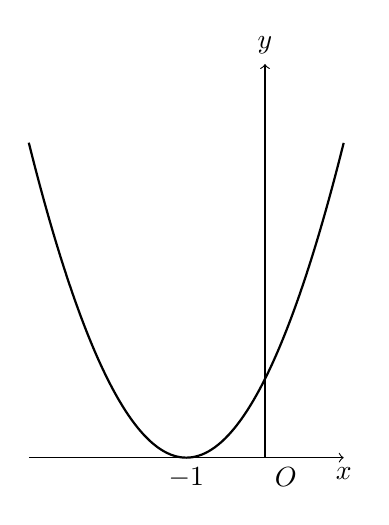
\begin{tikzpicture}
 \draw[->] (-3,0)--(1,0) node[below] {$x$};
 \draw[->] (0,0)--(0,5) node[above] {$y$};
 \draw[smooth,thick,samples=50,domain=-3:1] plot(\x,{(\x+1)*(\x+1)});
 \node[anchor=north west] at (0,0){$O$};
 \node[anchor=north] at (-1,0) {$-1$};
\end{tikzpicture}
\end{minipage}
\begin{minipage}{0.33\textwidth}
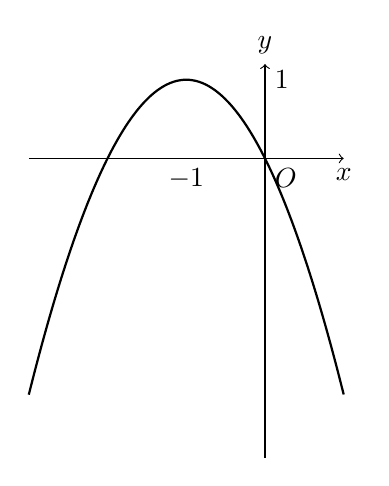
\begin{tikzpicture}
 \draw[->] (-3,0)--(1,0) node[below] {$x$};
 \draw[->] (0,-3.8)--(0,1.2) node[above] {$y$};
 \draw[smooth,thick,samples=50,domain=-3:1] plot(\x,{1-(\x+1)*(\x+1)});
 \node[anchor=north west] at (0,0){$O$};
 \node[anchor=north] at (-1,0) {$-1$};
 \node[anchor=west] at (0,1) {$1$};
\end{tikzpicture}
\end{minipage}
\caption{第1题中(1)、(2)、(3)的图像}
\label{fig:fun1}
\end{figure}

\begin{figure}[htbp]
\begin{minipage}{0.49\textwidth}
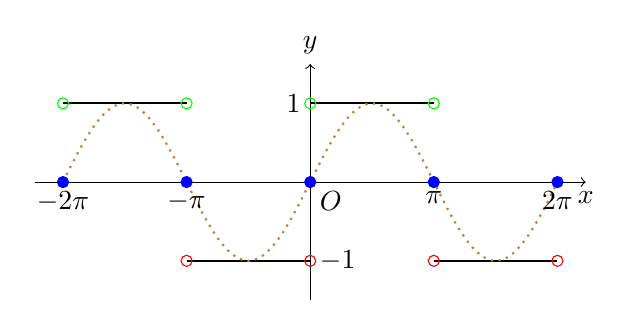
\begin{tikzpicture}
 \draw[->] (-3.5,0)--(3.5,0) node[below] {$x$};
 \draw[->] (0,-1.5)--(0,1.5) node[above] {$y$};
 \draw[smooth,thick,samples=50,domain=-3.14:-1.57] plot(\x,1);
  \draw[smooth,thick,samples=50,domain=-1.57:0] plot(\x,-1);
   \draw[smooth,thick,samples=50,domain=0:1.57] plot(\x,1);
    \draw[smooth,thick,samples=50,domain=1.57:3.14] plot(\x,-1);
   \draw[dotted,thick,brown,samples=100,domain=-3.14:3.14] plot(\x,{sin(2*\x r)});
 \node[anchor=north west] at (0,0){$O$};
 \node[anchor=east] at (0,1) {$1$};
 \node[anchor=west] at (0,-1) {$-1$};
 \filldraw[blue] (0,0) circle(2pt);
 \filldraw[blue] (1.57,0) circle(2pt);
 \filldraw[blue] (3.14,0) circle(2pt);
 \filldraw[blue] (-1.57,0) circle(2pt);
  \filldraw[blue] (-3.14,0) circle(2pt);
  \draw[green] (0,1) circle(2pt);
  \draw[green] (1.57,1) circle(2pt);
  \draw[green] (-1.57,1) circle(2pt);
  \draw[green] (-3.14,1) circle(2pt);
\draw[red] (0,-1) circle(2pt);
  \draw[red] (1.57,-1) circle(2pt);
  \draw[red] (-1.57,-1) circle(2pt);
  \draw[red] (3.14,-1) circle(2pt);
  \draw node[anchor=north] at (-3.14,0) {$-2\pi$};
  \draw node[anchor=north] at (-1.57,0) {$-\pi$};
  \draw node[anchor=north] at (3.14,0) {$2\pi$};
  \draw node[anchor=north] at (1.57,0) {$\pi$};
\end{tikzpicture}
\end{minipage}
\hfill
\begin{minipage}{0.49\textwidth}
\centering
\begin{tikzpicture}[scale=0.8]
 \draw[->] (-1.5,0)--(1.5,0) node[below] {$x$};
 \draw[->] (0,-4.5)--(0,4.5) node[above] {$y$};
 \draw[smooth,thick,samples=50,domain=-1:1] plot(\x,{(\x)^3});
 \draw[smooth,thick,samples=50,domain=-1.5:-1] plot(\x,{3*\x});
 \draw[smooth,thick,samples=50,domain=1:1.5] plot(\x,{3*\x});
 \node[anchor=north west] at (0,0){$O$};
 \node[anchor=south,scale=0.8] at (-1,0) {$-1$};
 \node[anchor=north,scale=0.8] at (1,0) {$1$};
 \node[anchor=west,scale=0.8] at (0,1) {$1$};
 \node[anchor=west,scale=0.8] at (0,3) {$3$};
 \node[anchor=east,scale=0.8] at (0,-1) {$-1$};
 \node[anchor=east,scale=0.8] at (0,-3) {$-3$};
 \filldraw[green] (1,3) circle(2pt);
 \filldraw[green] (-1,-3) circle(2pt);
 \draw[red] (1,1) circle(2pt);
 \draw[red] (-1,-1) circle(2pt);
\end{tikzpicture}
\end{minipage}
\caption{第1题中(4)、(5)的图像}
\label{fig:fun2}
\end{figure}
\begin{practice}
    试比较函数 $y=a^x$ 与 $y=\log_ax$ 分别当 $a=2$ 和 $a=\frac{1}{2}$ 时的图像.
\end{practice}

\begin{solve}
    绘制图像如\figref{fig:ax}所示.可见,$y=a^x$ 与 $y=\log_a x$ 总关于直线 $y=x$ 对称.事实上,互为反函数的函数的图像总是关于 $y=x$ 对称.
\end{solve}

\begin{figure}
    \centering
    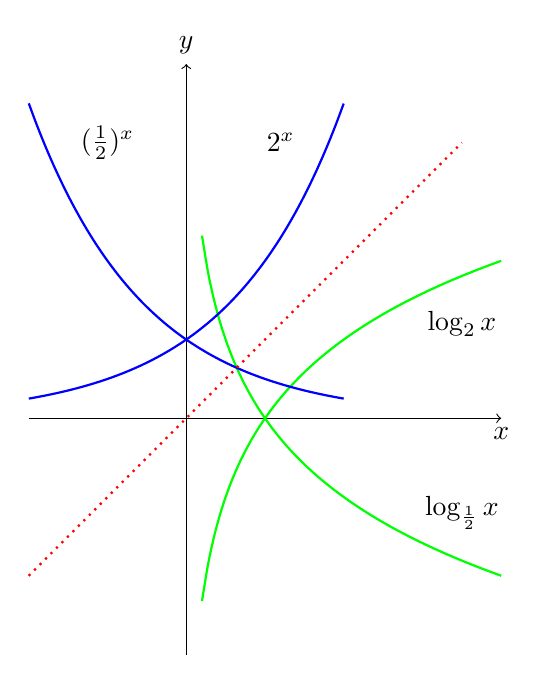
\begin{tikzpicture}
    \draw[->] (-2,0)--(4,0) node[below] {$x$};
 \draw[->] (0,-3)--(0,4.5) node[above] {$y$};
        \draw[green,smooth,thick,samples=50,domain=0.2:4] plot(\x,{ln(\x)/ln(2)});
 \draw[smooth,green,thick,samples=50,domain=0.2:4] plot(\x,{ln(\x)/ln(1/2)});
 \draw[smooth,blue,thick,samples=50,domain=-2:2] plot(\x,{2^\x});
 \draw[smooth,thick,blue,samples=50,domain=-2:2] plot(\x,{1/2^\x});
 \draw[smooth,thick,dotted,red,samples=50,domain=-2:3.5] plot(\x,{\x});

 \draw node at (3.5,1.2) {$\log_2 x$};
 \draw node at (3.5,-1.2) {$\log_{\frac{1}{2}} x$};
 \draw node at (1.2,3.5) {$2^x$};
 \draw node at (-1,3.5) {$(\frac{1}{2})^x$};
    \end{tikzpicture}
    \caption{$y=a^x$与$y=\log_a x$图像的比较}
    \label{fig:ax}
\end{figure}

\begin{practice}
    根据下图写出定义在 $[0,1]$ 上的分段函数 $f_1(x)$ 和 $f_2(x)$ 的解析式.
\begin{center}
    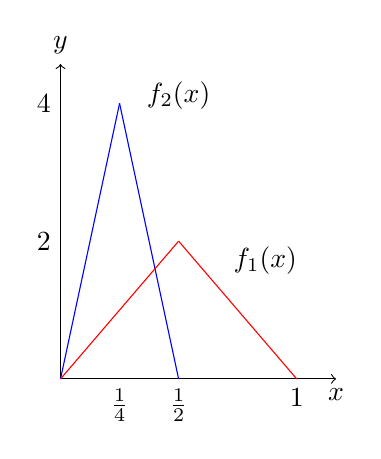
\begin{tikzpicture}
        \draw[->] (0,0)--(3.5,0) node[below] {$x$};
 \draw[->] (0,0)--(0,4) node[above] {$y$};
 \draw[blue] (0,0)--(3/4,3.5);
 \draw[blue] (3/4,3.5)--(1.5,0);
 \draw[red] (0,0)--(3/2,1.75);
 \draw[red] (3/2,1.75)--(3,0);
 \draw node[anchor=north] at (3/4,0) {$\frac{1}{4}$};
 \draw node[anchor=north] at (3/2,0) {$\frac{1}{2}$};
 \draw node[anchor=north] at (3,0) {$1$};
 \draw node[anchor=east] at (0,3.5) {$4$};
 \draw node[anchor=east] at (0,1.75) {$2$};
 \draw node at (3/2,3.6) {$f_2(x)$};
 \draw node at (2.6,1.5) {$f_1(x)$};
    \end{tikzpicture}
\end{center}
\end{practice}

\begin{solve}
    $$f_1(x)=\begin{cases}
        4x & 0\le x\le \frac{1}{2} \\
        -4x+4 & \frac{1}{2} < x \le 1
    \end{cases}$$
    $$f_2(x)=\begin{cases}
        16x & 0\le x\le \frac{1}{4} \\
        -16x+8 & \frac{1}{4} < x \le \frac{1}{2} \\
        0 & \frac{1}{2} < x \le 1
    \end{cases}$$

\quad
\end{solve}

\begin{practice}
    确定下列初等函数的存在域:

    (1) $y=\sin \sin x$ \qquad 
    (2) $y=\lg (\lg x)$

    (3) $y=\arcsin(\lg \frac{x}{10})$ \qquad 
    (4) $y=\lg (\arcsin \frac{x}{10})$
\end{practice}

\begin{solve}
    (1) 函数由 $y=\sin u,u\in \R$ 和 $u=\sin x,x\in \R$复合而成.函数的存在域为 $\setset{x\in \R}{\sin x\in \R}=\R$

    (2) 函数由 $y=\lg u,u\in (0,+\infty)$ 和 $u=\lg x,x\in (0,+\infty)$复合而成.函数的存在域为 $\setset{x\in (0,+\infty)}{\lg x\in (0,+\infty)}=(1,+\infty)$.

    (3) 函数由 $y=\arcsin u,u\in [-1,1]$ 和 $u=\lg \frac{x}{10},x\in (0,+\infty)$复合而成.函数的存在域为 $\setset{x\in (0,+\infty)}{\lg \frac{x}{10}\in [-1,1]}=[1,100]$.

    (4) 函数由 $y=\lg u,u\in (0,+\infty)$ 和 $u=\arcsin\frac{x}{10},x\in [-10,10]$复合而成.函数的存在域为 $\setset{x\in [-10,10]}{\arcsin \frac{x}{10}\in (0,+\infty)}=(0,10]$.
\end{solve}

\begin{practice}
    设函数 $f(x)=\begin{cases}
        2+x & x\le 0 \\
        2^x & x>0
    \end{cases}$.求:

    (1)$f(-3),f(0),f(1)$ \qquad (2) $f(\Delta x)-f(0),f(-\Delta x)-f(0)$.($\Delta x> 0$)
\end{practice}

\begin{solve}
    (1) $f(-3)=2+(-3)=-1$ \quad $f(0)=2+0=2$ \quad $f(1)=2^1=2$

    (2) $f(\Delta x)-f(0)=2^{\Delta x}-2$

    $f(-\Delta x)-f(0)=2-\Delta x-2=-\Delta x$
\end{solve}

\begin{practice}
    设函数 $f(x)=\frac{1}{1+x}$,求 $f(2+x),f(2x),f(x^2),f(f(x)),f(\frac{1}{f(x)})$.
\end{practice}

\begin{solve}
    \begin{align*}
        f(2+x)&= \frac{1}{1+(2+x)}=\frac{1}{3+x} \\
        f(2x)&= \frac{1}{1+2x} \\
        f(x^2)&= \frac{1}{1+x^2}\\
        f(f(x))&= \frac{1}{1+\frac{1}{1+x}}=\frac{1+x}{2+x} \\
        f(\frac{1}{f(x)})&=f(1+x)=\frac{1}{1+(1+x)}=\frac{1}{2+x}
    \end{align*}
    \quad
\end{solve}

\begin{practice}
    试问下列函数是由哪些初等函数复合而成:
    
(1) $y=(1+x)^{20}$ \quad (2) $y=(\arcsin x^2)^2$

(3) $y=\lg (1+\sqrt{1+x^2})$ \quad (4) $y=2^{\sin^2 x}$
\end{practice}

\begin{solve}
    (1) 函数由 $y=u^{20}$, $u=v+w$,$v=1$,$w=x$ 复合而成.

    (2) 函数由 $y=u^{2}$, $u=\arcsin v$ 和 $v=x^2$ 复合而成.

    (3) 函数由 $y=\lg u$, $u=v+w$, 
    $v=1$,$w=s^{\frac{1}{2}}$,$s=v+t$,$t=x^2$复合而成.

    (3) 函数由 $y=2^u$, $u=v^2$, 
    $v=\sin x$ 复合而成.
\end{solve}

\begin{practice}
    在什么条件下,函数 $y=\frac{ax+b}{cx+d}$ 的反函数就是它本身?
\end{practice}

\begin{solve}
(1) 若 $c=0$,则$d\ne 0$,则原函数为 $y=\frac{a}{d}x+\frac{b}{d}$

若反函数存在,则 $a\ne 0$,反解得 $x=\frac{d}{a}y-\frac{b}{a}$.

如果反函数就是它本身,则 $\frac{d}{a}=\frac{a}{d},\frac{b}{d}=-\frac{b}{a}\iff a^2=d^2,b(a+d)=0$

因此, $c=0,a\ne 0,a=d,b=0$ 或 $c=0,a\ne 0,a=-d$ 时,函数的反函数就是它本身.

(2) 若$c\ne 0$,则原函数为 $y=\frac{ax+b}{cx+d},x\ne -\frac{d}{c}$

    若$\frac{a}{c}\ne \frac{b}{d}$,则反函数存在.反解得 $x=\frac{-yd+b}{cy-a},y\ne \frac{a}{c}$.

如果反函数就是它本身,则 $a=-d$.

因此,$
c\ne 0,ad\ne bc,a=-d$时,函数的反函数就是它本身.
\end{solve}

\begin{practice}
    试作函数 $y=\arcsin(\sin x)$ 的图像.
\end{practice}

\begin{figure}[htbp]
    \centering
    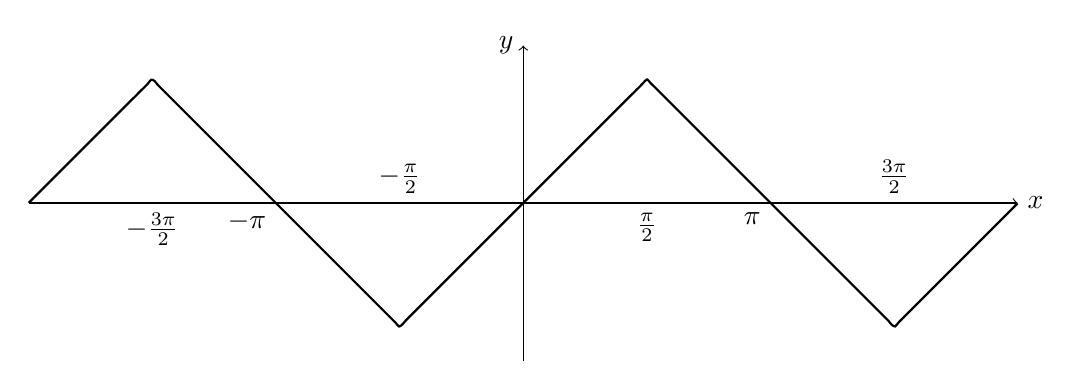
\begin{tikzpicture}
        \draw[->,right] (-6.28,0)--(6.28,0) node {$x$};
        \draw[->,left] (0,-2)--(0,2) node {$y$};
        \draw[thick,smooth,samples=300,domain=-6.28:6.28] plot(\x,{rad(asin(sin(\x r)))});

        \draw[below] node at (-1.57*3,0) {$-\frac{3\pi}{2}$};
        \draw node[anchor=north east] at (-1.57*2,0) {$-\pi$};
        \draw node[anchor=south] at (-1.57,0) {$-\frac{\pi}{2}$};
        \draw node[anchor=south] at (1.57*3,0) {$\frac{3\pi}{2}$};
        \draw node[anchor=north east]  at (1.57*2,0){$\pi$};
        \draw node[anchor=north] at (1.57,0) {$\frac{\pi}{2}$};
    \end{tikzpicture}
    \caption{函数 $y=\arcsin(\sin x)$ 的图像}
    \label{fig:arcsin}
\end{figure}

\begin{solve}
    在 $[-\frac{\pi}{2},\frac{\pi}{2}]$ 上 ,$y=\arcsin(\sin x)=x$. 

    而当 $x\in [\frac{\pi}{2},\frac{3\pi}{2}]$ 时,有 $\pi-x \in [-\frac{\pi}{2},\frac{\pi}{2}]$,
    
    故 $y=\arcsin(\sin x)=\arcsin(\sin(\pi- x))=\pi-x$.

    当 $x\in [\frac{3\pi}{2},\frac{5\pi}{2}]$ 时,有 $x-2\pi \in [-\frac{\pi}{2},\frac{\pi}{2}]$,
    
    故 $y=\arcsin(\sin x)=\arcsin(\sin(x-2\pi))=x-2\pi$.

    可归纳得 $y=\arcsin(\sin x)=(-1)^k(x-k\pi),x\in [-\frac{\pi}{2}+k\pi,\frac{\pi}{2}+k\pi],k\in \mathbb{Z}$
\end{solve}

\begin{practice}
    试问下列等式是否成立:
    
    (1) $\tan (\arctan x)=x,x\in \R$
    
    (2) $\arctan (\tan x)=x,x\ne \frac{\pi}{2}+k\pi,k=0,\pm 1,\pm 2,+\infty$
\end{practice}

\begin{solve}
    (1) 成立.

    (2) 不成立. 在 $(-\frac{\pi}{2},\frac{\pi}{2})$ 上确实有 $\arctan(\tan x)=x$.但在 $(\frac{\pi}{2},\frac{3\pi}{2})$ 上,有 $x-\pi \in (-\frac{\pi}{2},\frac{\pi}{2})$,则 $\arctan(\tan x)=\arctan(\tan (x-\pi))=x-\pi$.同理可得,在 $(-\frac{\pi}{2}+k\pi,\frac{\pi}{2}+k\pi)$ 上,有 $\arctan(\tan x)=\arctan(\tan (x-k\pi))=x-k\pi$
\end{solve}

\begin{practice}
    试问 $y=\abs{x}$ 是初等函数吗?
\end{practice}

\begin{solve}
    是. $y=\abs{x}=\sqrt{x^2}$ 由基本初等函数 $y=u^{\frac{1}{2}}$ 和 $u=x^2$ 复合而成.
\end{solve}

\begin{practice}
    证明关于函数 $y=\lfloor x \rfloor$ 的如下不等式:

    (1) 当 $x>0$ 时,$1-x<x\lfloor \frac{1}{x} \rfloor \le 1$.

    (2) 当 $x<0$时,$1\le x\lfloor \frac{1}{x} \rfloor <1-x$.
\end{practice}

\begin{proof}
    (1) 当 $x>0$ 时,有 $ \frac{1}{x}  -1 < \lfloor \frac{1}{x} \rfloor\le \frac{1}{x}$,两边同乘 $x$,得到 $1-x<x\lfloor \frac{1}{x} \rfloor \le 1$.

   (2) 当 $x<0$ 时,同样有 $ \frac{1}{x}  -1 < \lfloor \frac{1}{x} \rfloor\le \frac{1}{x}$,两边同乘 $x$,得到 $1\le x\lfloor \frac{1}{x} \rfloor < 1-x$.
\end{proof}

\newsection